\documentclass[10pt]{beamer}

% \usetheme[progressbar=frametitle]{metropolis}
\usetheme{metropolis}

\definecolor{inf_primary}{RGB}{0, 0, 0}
\definecolor{inf_secondary}{RGB}{237, 28, 36}
\definecolor{inf_tertiary}{RGB}{147, 149, 152}

\setbeamercolor{normal text}{fg=inf_primary}
\setbeamercolor{alerted text}{fg=inf_secondary}

\usepackage{appendixnumberbeamer}

\usepackage{booktabs}
\usepackage[scale=2]{ccicons}

\usepackage{pgfplots}
\usepgfplotslibrary{dateplot}

\usepackage{xspace}
\usepackage{cancel}
\usepackage{array}
\usepackage{lipsum}
\usepackage{graphicx}

\usepackage[authoryear]{natbib}

\usepackage{tikz}
\usetikzlibrary{positioning, arrows.meta, patterns, automata}

\title{Understanding Sample Generation\\Strategies for Learning Heuristic\\Functions in Classical Planning}
\date{}
\author{Author: Rafael Vales Bettker\\Advisor: Prof. Dr. Andr\'{e} Grahl Pereira\\Co-advisor: Prof. Dr. Marcus Ritt}
\institute{Federal University of Rio Grande do Sul (UFRGS)\\Institute of Informatics\\Department of Theoretical Informatics}

\newcommand{\drawblock}[5]{% PARAMETERS: COLOR, CORNERCOORDS, SIZE
% TOP SIDE
\color{#1!55}
\pgfmoveto{\pgfrelative{\pgfxyz(#2,#3,#4)}{\pgfxyz(0,#5,0)}}
\pgflineto{\pgfrelative{\pgfxyz(#2,#3,#4)}{\pgfxyz(#5,#5,0)}}
\pgflineto{\pgfrelative{\pgfxyz(#2,#3,#4)}{\pgfxyz(#5,#5,#5)}}
\pgflineto{\pgfrelative{\pgfxyz(#2,#3,#4)}{\pgfxyz(0,#5,#5)}}
\pgflineto{\pgfrelative{\pgfxyz(#2,#3,#4)}{\pgfxyz(0,#5,0)}}
\pgffill
\color{black}
\pgfmoveto{\pgfrelative{\pgfxyz(#2,#3,#4)}{\pgfxyz(0,#5,0)}}
\pgflineto{\pgfrelative{\pgfxyz(#2,#3,#4)}{\pgfxyz(#5,#5,0)}}
\pgflineto{\pgfrelative{\pgfxyz(#2,#3,#4)}{\pgfxyz(#5,#5,#5)}}
\pgflineto{\pgfrelative{\pgfxyz(#2,#3,#4)}{\pgfxyz(0,#5,#5)}}
\pgflineto{\pgfrelative{\pgfxyz(#2,#3,#4)}{\pgfxyz(0,#5,0)}}
\pgfstroke
% RIGHT SIDE
\color{#1!65}
\pgfmoveto{\pgfrelative{\pgfxyz(#2,#3,#4)}{\pgfxyz(#5,0,0)}}
\pgflineto{\pgfrelative{\pgfxyz(#2,#3,#4)}{\pgfxyz(#5,#5,0)}}
\pgflineto{\pgfrelative{\pgfxyz(#2,#3,#4)}{\pgfxyz(#5,#5,#5)}}
\pgflineto{\pgfrelative{\pgfxyz(#2,#3,#4)}{\pgfxyz(#5,0,#5)}}
\pgflineto{\pgfrelative{\pgfxyz(#2,#3,#4)}{\pgfxyz(#5,0,0)}}
\pgffill
\color{black}
\pgfmoveto{\pgfrelative{\pgfxyz(#2,#3,#4)}{\pgfxyz(#5,0,0)}}
\pgflineto{\pgfrelative{\pgfxyz(#2,#3,#4)}{\pgfxyz(#5,#5,0)}}
\pgflineto{\pgfrelative{\pgfxyz(#2,#3,#4)}{\pgfxyz(#5,#5,#5)}}
\pgflineto{\pgfrelative{\pgfxyz(#2,#3,#4)}{\pgfxyz(#5,0,#5)}}
\pgflineto{\pgfrelative{\pgfxyz(#2,#3,#4)}{\pgfxyz(#5,0,0)}}
\pgfstroke
%FRONT
\color{#1!99}
\pgfmoveto{\pgfxyz(#2,#3,#4)}
\pgflineto{\pgfrelative{\pgfxyz(#2,#3,#4)}{\pgfxyz(#5,0,0)}}
\pgflineto{\pgfrelative{\pgfxyz(#2,#3,#4)}{\pgfxyz(#5,#5,0)}}
\pgflineto{\pgfrelative{\pgfxyz(#2,#3,#4)}{\pgfxyz(0,#5,0)}}
\pgflineto{\pgfxyz(#2,#3,#4)}
\pgffill
\color{black}
\pgfmoveto{\pgfxyz(#2,#3,#4)}
\pgflineto{\pgfrelative{\pgfxyz(#2,#3,#4)}{\pgfxyz(#5,0,0)}}
\pgflineto{\pgfrelative{\pgfxyz(#2,#3,#4)}{\pgfxyz(#5,#5,0)}}
\pgflineto{\pgfrelative{\pgfxyz(#2,#3,#4)}{\pgfxyz(0,#5,0)}}
\pgflineto{\pgfxyz(#2,#3,#4)}
\pgfstroke
}

\newcommand{\RsGsB}{\begin{pgfpicture}{0.5mm}{0.5mm}{9mm}{3.75mm}
\pgfsetxvec{\pgfpoint{0.4cm}{0cm}}
\pgfsetyvec{\pgfpoint{0cm}{0.4cm}}
\pgfsetzvec{\pgfpoint{0.15cm}{0.15cm}}
\drawblock{red}{0}{0}{0}{0.75}
\drawblock{green}{0.75}{0}{0}{0.75}
\drawblock{blue}{1.5}{0}{0}{0.75}
\end{pgfpicture}
}

\newcommand{\twostacksA}[3]{\begin{pgfpicture}{0.5mm}{0.5mm}{0.6cm}{0.675cm}
\pgfsetxvec{\pgfpoint{0.4cm}{0cm}}
\pgfsetyvec{\pgfpoint{0cm}{0.4cm}}
\pgfsetzvec{\pgfpoint{0.15cm}{0.15cm}}
\drawblock{#2}{0}{0}{0}{0.75}
\drawblock{#1}{0}{0.75}{0}{0.75}
\drawblock{#3}{0.75}{0}{0}{0.75}
\end{pgfpicture}
}

\newcommand{\twostacksB}[3]{\begin{pgfpicture}{0.5mm}{0.5mm}{0.6cm}{0.675cm}
\pgfsetxvec{\pgfpoint{0.4cm}{0cm}}
\pgfsetyvec{\pgfpoint{0cm}{0.4cm}}
\pgfsetzvec{\pgfpoint{0.15cm}{0.15cm}}
\drawblock{#1}{0}{0}{0}{0.75}
\drawblock{#3}{0.75}{0}{0}{0.75}
\drawblock{#2}{0.75}{0.75}{0}{0.75}
\end{pgfpicture}
}

\newcommand{\onestack}[3]{\begin{pgfpicture}{0.5mm}{0.5mm}{3mm}{9.75mm}
\pgfsetxvec{\pgfpoint{0.4cm}{0cm}}
\pgfsetyvec{\pgfpoint{0cm}{0.4cm}}
\pgfsetzvec{\pgfpoint{0.15cm}{0.15cm}}
\drawblock{#3}{0}{0}{0}{0.75}
\drawblock{#2}{0}{0.75}{0}{0.75}
\drawblock{#1}{0}{1.5}{0}{0.75}
\end{pgfpicture}
}

\newcommand{\RGsB}{\twostacksA{red}{green}{blue}}

\newcommand{\RBsG}{\twostacksB{green}{red}{blue}}
\newcommand{\RBsGr}{\twostacksA{red}{blue}{green}}

\newcommand{\BRsG}{\twostacksA{blue}{red}{green}}
\newcommand{\BRsGr}{\twostacksB{green}{blue}{red}}

\newcommand{\RsBG}{\twostacksB{red}{blue}{green}}

\newcommand{\GRsB}{\twostacksA{green}{red}{blue}}
\newcommand{\RsGB}{\twostacksB{red}{green}{blue}}

\newcommand{\RGB}{\onestack{red}{green}{blue}}
\newcommand{\RBG}{\onestack{red}{blue}{green}}
\newcommand{\GRB}{\onestack{green}{red}{blue}}
\newcommand{\GBR}{\onestack{green}{blue}{red}}
\newcommand{\BRG}{\onestack{blue}{red}{green}}
\newcommand{\BGR}{\onestack{blue}{green}{red}}


% TRANSPARENT BLOCK
\newcommand{\drawblockt}[5]{% PARAMETERS: COLOR, CORNERCOORDS, SIZE
% TOP SIDE
\color{#1!18}
\pgfmoveto{\pgfrelative{\pgfxyz(#2,#3,#4)}{\pgfxyz(0,#5,0)}}
\pgflineto{\pgfrelative{\pgfxyz(#2,#3,#4)}{\pgfxyz(#5,#5,0)}}
\pgflineto{\pgfrelative{\pgfxyz(#2,#3,#4)}{\pgfxyz(#5,#5,#5)}}
\pgflineto{\pgfrelative{\pgfxyz(#2,#3,#4)}{\pgfxyz(0,#5,#5)}}
\pgflineto{\pgfrelative{\pgfxyz(#2,#3,#4)}{\pgfxyz(0,#5,0)}}
\pgffill
\color{black!33}
\pgfmoveto{\pgfrelative{\pgfxyz(#2,#3,#4)}{\pgfxyz(0,#5,0)}}
\pgflineto{\pgfrelative{\pgfxyz(#2,#3,#4)}{\pgfxyz(#5,#5,0)}}
\pgflineto{\pgfrelative{\pgfxyz(#2,#3,#4)}{\pgfxyz(#5,#5,#5)}}
\pgflineto{\pgfrelative{\pgfxyz(#2,#3,#4)}{\pgfxyz(0,#5,#5)}}
\pgflineto{\pgfrelative{\pgfxyz(#2,#3,#4)}{\pgfxyz(0,#5,0)}}
\pgfstroke
% RIGHT SIDE
\color{#1!22}
\pgfmoveto{\pgfrelative{\pgfxyz(#2,#3,#4)}{\pgfxyz(#5,0,0)}}
\pgflineto{\pgfrelative{\pgfxyz(#2,#3,#4)}{\pgfxyz(#5,#5,0)}}
\pgflineto{\pgfrelative{\pgfxyz(#2,#3,#4)}{\pgfxyz(#5,#5,#5)}}
\pgflineto{\pgfrelative{\pgfxyz(#2,#3,#4)}{\pgfxyz(#5,0,#5)}}
\pgflineto{\pgfrelative{\pgfxyz(#2,#3,#4)}{\pgfxyz(#5,0,0)}}
\pgffill
\color{black!33}
\pgfmoveto{\pgfrelative{\pgfxyz(#2,#3,#4)}{\pgfxyz(#5,0,0)}}
\pgflineto{\pgfrelative{\pgfxyz(#2,#3,#4)}{\pgfxyz(#5,#5,0)}}
\pgflineto{\pgfrelative{\pgfxyz(#2,#3,#4)}{\pgfxyz(#5,#5,#5)}}
\pgflineto{\pgfrelative{\pgfxyz(#2,#3,#4)}{\pgfxyz(#5,0,#5)}}
\pgflineto{\pgfrelative{\pgfxyz(#2,#3,#4)}{\pgfxyz(#5,0,0)}}
\pgfstroke
%FRONT
\color{#1!33}
\pgfmoveto{\pgfxyz(#2,#3,#4)}
\pgflineto{\pgfrelative{\pgfxyz(#2,#3,#4)}{\pgfxyz(#5,0,0)}}
\pgflineto{\pgfrelative{\pgfxyz(#2,#3,#4)}{\pgfxyz(#5,#5,0)}}
\pgflineto{\pgfrelative{\pgfxyz(#2,#3,#4)}{\pgfxyz(0,#5,0)}}
\pgflineto{\pgfxyz(#2,#3,#4)}
\pgffill
\color{black!33}
\pgfmoveto{\pgfxyz(#2,#3,#4)}
\pgflineto{\pgfrelative{\pgfxyz(#2,#3,#4)}{\pgfxyz(#5,0,0)}}
\pgflineto{\pgfrelative{\pgfxyz(#2,#3,#4)}{\pgfxyz(#5,#5,0)}}
\pgflineto{\pgfrelative{\pgfxyz(#2,#3,#4)}{\pgfxyz(0,#5,0)}}
\pgflineto{\pgfxyz(#2,#3,#4)}
\pgfstroke
}

\newcommand{\RsGsBt}{\begin{pgfpicture}{0.5mm}{0.5mm}{9mm}{3.75mm}
\pgfsetxvec{\pgfpoint{0.4cm}{0cm}}
\pgfsetyvec{\pgfpoint{0cm}{0.4cm}}
\pgfsetzvec{\pgfpoint{0.15cm}{0.15cm}}
\drawblockt{red}{0}{0}{0}{0.75}
\drawblockt{green}{0.75}{0}{0}{0.75}
\drawblockt{blue}{1.5}{0}{0}{0.75}
\end{pgfpicture}
}

\newcommand{\twostacksAt}[3]{\begin{pgfpicture}{0.5mm}{0.5mm}{0.6cm}{0.675cm}
\pgfsetxvec{\pgfpoint{0.4cm}{0cm}}
\pgfsetyvec{\pgfpoint{0cm}{0.4cm}}
\pgfsetzvec{\pgfpoint{0.15cm}{0.15cm}}
\drawblockt{#2}{0}{0}{0}{0.75}
\drawblockt{#1}{0}{0.75}{0}{0.75}
\drawblockt{#3}{0.75}{0}{0}{0.75}
\end{pgfpicture}
}

\newcommand{\twostacksBt}[3]{\begin{pgfpicture}{0.5mm}{0.5mm}{0.6cm}{0.675cm}
\pgfsetxvec{\pgfpoint{0.4cm}{0cm}}
\pgfsetyvec{\pgfpoint{0cm}{0.4cm}}
\pgfsetzvec{\pgfpoint{0.15cm}{0.15cm}}
\drawblockt{#1}{0}{0}{0}{0.75}
\drawblockt{#3}{0.75}{0}{0}{0.75}
\drawblockt{#2}{0.75}{0.75}{0}{0.75}
\end{pgfpicture}
}

\newcommand{\onestackt}[3]{\begin{pgfpicture}{0.5mm}{0.5mm}{3mm}{9.75mm}
\pgfsetxvec{\pgfpoint{0.4cm}{0cm}}
\pgfsetyvec{\pgfpoint{0cm}{0.4cm}}
\pgfsetzvec{\pgfpoint{0.15cm}{0.15cm}}
\drawblockt{#3}{0}{0}{0}{0.75}
\drawblockt{#2}{0}{0.75}{0}{0.75}
\drawblockt{#1}{0}{1.5}{0}{0.75}
\end{pgfpicture}
}

\newcommand{\RGsBt}{\twostacksAt{red}{green}{blue}}

\newcommand{\RBsGt}{\twostacksBt{green}{red}{blue}}
\newcommand{\RBsGrt}{\twostacksAt{red}{blue}{green}}

\newcommand{\BRsGt}{\twostacksAt{blue}{red}{green}}
\newcommand{\BRsGrt}{\twostacksBt{green}{blue}{red}}

\newcommand{\RsBGt}{\twostacksBt{red}{blue}{green}}

\newcommand{\GRsBt}{\twostacksAt{green}{red}{blue}}
\newcommand{\RsGBt}{\twostacksBt{red}{green}{blue}}

\newcommand{\RGBt}{\onestackt{red}{green}{blue}}
\newcommand{\RBGt}{\onestackt{red}{blue}{green}}
\newcommand{\GRBt}{\onestackt{green}{red}{blue}}
\newcommand{\GBRt}{\onestackt{green}{blue}{red}}
\newcommand{\BRGt}{\onestackt{blue}{red}{green}}
\newcommand{\BGRt}{\onestackt{blue}{green}{red}}

\newcommand{\email}[1]{\href{mailto:#1}{#1}}

\providecommand{\ssdiameter}{\ensuremath{d^*}\xspace}
\providecommand{\facts}{\ensuremath{F}\xspace}
\providecommand{\meanfx}{\ensuremath{\bar F}\xspace}
\providecommand{\default}{\ensuremath{200}\xspace}

\providecommand{\h}{\ensuremath{h}\xspace}
\providecommand{\hvalue}[1]{\ensuremath{h^{#1}}\xspace}
\providecommand{\hstar}{\hvalue{*}}
\providecommand{\hff}{\hvalue{\text{FF}}}
\providecommand{\hgc}{\hvalue{\text{GC}}}
\providecommand{\hnnbase}{\ensuremath{\hat h_{0}}\xspace}
\providecommand{\hnnl}[1]{\ensuremath{\hat h_{#1}}\xspace}
\providecommand{\hnnrsp}[1]{\ensuremath{\hat h{^{#1\%}_\text{\meanfx}}}\xspace}
\providecommand{\hnnrs}{\hnnrsp{20}}
\providecommand{\hnrsl}{\ensuremath{\hat h^{\text{N-RSL}}}\xspace}
\providecommand{\hboot}{\ensuremath{\hat h^{\text{Boot}}}\xspace}

\providecommand{\ceil}[1]{\ensuremath{\left\lceil #1\right\rceil}}

\newcommand\blfootnote[1]{%
  \begingroup
  \renewcommand\thefootnote{}\footnote{#1}%
  \addtocounter{footnote}{-1}%
  \endgroup
}

\begin{document}

\maketitle

\begin{frame}{Table of contents}
  \setbeamertemplate{section in toc}[sections numbered]
  \tableofcontents[hideallsubsections]
\end{frame}

%%%%%%%%%%%%%%%%%%%%%%%%
\section{Introduction}

\begin{frame}{Introduction}
\begin{itemize}
    \item Classical planning provides a method for representing and solving various problems.
    \item Planning tasks are typically defined by the initial state and the desired outcome (goal state).
    \item Heuristic functions guide search algorithms to find solutions.
    \item Learning heuristic functions with neural networks (NN) based on samples that are states with their cost-to-goal estimates.
    \begin{itemize}
        \item The NN is our \alert{heuristic function} and solves distinct initial states of a state space.
    \end{itemize}
\end{itemize}
\end{frame}

\begin{frame}{Problem and Contributions}
    Learn effective NN-based heuristic functions.
    \begin{itemize}
        \item How to generate good samples?
        \item What is relevant to the quality of the samples?
    \end{itemize}
    \bigskip
    \pause
    Our contributions include
    \begin{itemize}
        \item A systematic study of sampling strategies.
        \item New sampling and \h-value refinement algorithms.
    \end{itemize}
\end{frame}

%%%%%%%%%%%%%%%%%%%%%%%%
\section{Background}

\subsection{Classical Planning}

\begin{frame}{Classical Planning}
    \only<-2> {
        A planning task can be defined as a tuple~$\Pi=\langle\mathcal{S},\mathcal{O},s_0,s^*,\text{cost}\rangle$.
    }
    \only<3> {
        A planning task can be defined as a tuple~$\Pi=\langle\alert{\mathcal{S}},\mathcal{O},s_0,s^*,\text{cost}\rangle$.
    }
    \only<4> {
        A planning task can be defined as a tuple~$\Pi=\langle\mathcal{S},\alert{\mathcal{O}},s_0,s^*,\text{cost}\rangle$.
    }
    \only<6> {
        A planning task can be defined as a tuple~$\Pi=\langle\mathcal{S},\mathcal{O},\alert{s_0},s^*,\text{cost}\rangle$.
    }
    \only<7> {
        A planning task can be defined as a tuple~$\Pi=\langle\mathcal{S},\mathcal{O},s_0,\alert{s^*},\text{cost}\rangle$.
    }
    \only<5> {
        A planning task can be defined as a tuple~$\Pi=\langle\mathcal{S},\mathcal{O},s_0,s^*,\alert{\text{cost}}\rangle$.
    }
    \only<8-> {
        A planning task can be defined as a tuple~$\Pi=\langle\mathcal{S},\mathcal{O},s_0,s^*,\text{cost}\rangle$.
    }

    \only<3-> { \bigskip }

    \only<1> {
        \vspace{5.06cm}
    }
    \only<2-> {
        \centering
        \begin{pgfpicture}{-29.25mm}{-24.3mm}{29.25mm}{24.3mm}
            \only<3> {
                \pgfnodebox{RBG}[virtual]{\pgfpolar{180}{24mm}}{\RBG}{1.5pt}{1.5pt}
                \pgfnodebox{RsBG}[virtual]{\pgfpolar{180}{12mm}}{\RsBG}{1.5pt}{1.5pt}
                \pgfnodebox{BRsG}[virtual]{\pgfpolar{120}{12mm}}{\BRsG}{1.5pt}{1.5pt}
                \pgfnodebox{RsGsB}[virtual]{\pgfpolar{0}{0cm}}{\RsGsB}{1.5pt}{1.5pt}
                \pgfnodebox{GBR}[virtual]{\pgfpolar{130}{24mm}}{\GBR}{1.5pt}{1.5pt}
                \pgfnodebox{GRsB}[virtual]{\pgfpolar{300}{12mm}}{\GRsB}{1.5pt}{1.5pt}
                \pgfnodebox{BGR}[virtual]{\pgfpolar{310}{24mm}}{\BGR}{1.5pt}{1.5pt}
                \pgfnodebox{RGsB}[virtual]{\pgfpolar{0}{12mm}}{\RGsB}{1.5pt}{1.5pt}
                \pgfnodebox{RBsG}[virtual]{\pgfpolar{60}{12mm}}{\RBsG}{1.5pt}{1.5pt}
                \pgfnodebox{RsGB}[virtual]{\pgfpolar{240}{12mm}}{\RsGB}{1.5pt}{1.5pt}
                \pgfnodebox{BRG}[virtual]{\pgfpolar{0}{24mm}}{\BRG}{1.5pt}{1.5pt}
                \pgfnodebox{GRB}[virtual]{\pgfpolar{50}{24mm}}{\GRB}{1.5pt}{1.5pt}
                \pgfnodebox{RGB}[virtual]{\pgfpolar{230}{24mm}}{\RGB}{1.5pt}{1.5pt}
            }
            \only<-2,4-> {
                \only<6,8> {
                    \pgfnodebox{RBG}[virtual]{\pgfpolar{180}{24mm}}{\RBG}{1.5pt}{1.5pt}
                }
                \only<-5,7> {
                    \pgfnodebox{RBG}[virtual]{\pgfpolar{180}{24mm}}{\RBGt}{1.5pt}{1.5pt}
                }
                \only<7,8> {
                    \pgfnodebox{BGR}[virtual]{\pgfpolar{310}{24mm}}{\BGR}{1.5pt}{1.5pt}
                }
                \only<-6> {
                    \pgfnodebox{BGR}[virtual]{\pgfpolar{310}{24mm}}{\BGRt}{1.5pt}{1.5pt}
                }
                \only<8> {
                    \pgfnodebox{RsBG}[virtual]{\pgfpolar{180}{12mm}}{\RsBG}{1.5pt}{1.5pt}
                    \pgfnodebox{RsGsB}[virtual]{\pgfpolar{0}{0cm}}{\RsGsB}{1.5pt}{1.5pt}
                    \pgfnodebox{RsGB}[virtual]{\pgfpolar{240}{12mm}}{\RsGB}{1.5pt}{1.5pt}
                    \pgfnodebox{GRsB}[virtual]{\pgfpolar{300}{12mm}}{\GRsB}{1.5pt}{1.5pt}
                }
                \only<-7> {
                    \pgfnodebox{RsBG}[virtual]{\pgfpolar{180}{12mm}}{\RsBGt}{1.5pt}{1.5pt}
                    \pgfnodebox{RsGsB}[virtual]{\pgfpolar{0}{0cm}}{\RsGsBt}{1.5pt}{1.5pt}
                    \pgfnodebox{RsGB}[virtual]{\pgfpolar{240}{12mm}}{\RsGBt}{1.5pt}{1.5pt}
                    \pgfnodebox{GRsB}[virtual]{\pgfpolar{300}{12mm}}{\GRsBt}{1.5pt}{1.5pt}
                }
                \pgfnodebox{BRsG}[virtual]{\pgfpolar{120}{12mm}}{\BRsGt}{1.5pt}{1.5pt}
                \pgfnodebox{GBR}[virtual]{\pgfpolar{130}{24mm}}{\GBRt}{1.5pt}{1.5pt}
                \pgfnodebox{RGsB}[virtual]{\pgfpolar{0}{12mm}}{\RGsBt}{1.5pt}{1.5pt}
                \pgfnodebox{RBsG}[virtual]{\pgfpolar{60}{12mm}}{\RBsGt}{1.5pt}{1.5pt}
                \pgfnodebox{BRG}[virtual]{\pgfpolar{0}{24mm}}{\BRGt}{1.5pt}{1.5pt}
                \pgfnodebox{GRB}[virtual]{\pgfpolar{50}{24mm}}{\GRBt}{1.5pt}{1.5pt}
                \pgfnodebox{RGB}[virtual]{\pgfpolar{230}{24mm}}{\RGBt}{1.5pt}{1.5pt}
            }
            \only<4,5> {
                \pgfsetarrowsend{Triangle[scale=0.8pt]}
                \pgfsetstrokecolor{black}
                \pgfnodeconnline{RsBG}{BRsG}
                \pgfnodeconnline{GBR}{BRsG}
                \pgfnodeconnline{GRsB}{RsGsB}
                \pgfnodeconnline{BGR}{GRsB}
                \pgfnodeconnline{RGsB}{RsGsB}
                \pgfnodeconnline{BRsG}{RsGsB}
                \pgfnodeconnline{RsGB}{RsGsB}
                \pgfnodeconnline{BRG}{RGsB}
                \pgfnodeconnline{GRB}{RBsG}
                \pgfnodeconnline{RGB}{RsGB}
                \pgfnodeconnline{RBsG}{RGsB}
                \pgfnodeconnline{GRsB}{RsGB}
                \pgfnodeconnline{RsBG}{RBG}
                \pgfnodeconnline{RsGsB}{RsBG}
                \pgfnodeconnline{RBsG}{RsGsB}
            }
            \only<-3,6-> {
                \pgfsetstrokecolor{lightgray}
            }
            \pgfnodeconnline{BRsG}{RsBG}
            \pgfnodeconnline{BRsG}{GBR}
            \pgfnodeconnline{RsGsB}{GRsB}
            \pgfnodeconnline{RsGsB}{RGsB}
            \pgfnodeconnline{RsGsB}{BRsG}
            \pgfnodeconnline{RGsB}{BRG}
            \pgfnodeconnline{RBsG}{GRB}
            \pgfnodeconnline{RsGB}{RGB}
            \pgfnodeconnline{RGsB}{RBsG}
            \pgfnodeconnline{RsGsB}{RBsG}
            \only<8> {
                \pgfsetarrowsend{Triangle[scale=0.8pt]}
                \pgfsetstrokecolor{black}
                \pgfnodeconnline{RBG}{RsBG}
                \pgfnodeconnline{RsBG}{RsGsB}
                \pgfnodeconnline{RsGsB}{RsGB}
                \pgfnodeconnline{RsGB}{GRsB}
                \pgfnodeconnline{GRsB}{BGR}
            }
            \only<-7> {
                \pgfnodeconnline{RBG}{RsBG}
                \pgfnodeconnline{RsBG}{RsGsB}
                \pgfnodeconnline{RsGsB}{RsGB}
                \pgfnodeconnline{RsGB}{GRsB}
                \pgfnodeconnline{GRsB}{BGR}
            }
        \end{pgfpicture}
    }
\end{frame}

\subsection{Related Work}

\begin{frame}{Related Work}
\begin{columns}
    \begin{column}{0.5\textwidth}
        Structured NN-based
        \newline
        \begin{itemize}
            \item Structured neural networks.
            \item Encode part of the model into the network architecture.
            \item Tipically multi-domain or domain-independent.
            \item E.g. \citet{shen2020learning}
        \end{itemize}
    \end{column}
    \begin{column}{0.5\textwidth}
        Non-structured NN-based
        \newline
        \begin{itemize}
            \item Feedforward neural networks.
            \item Highly independent of the task description. 
            \item Typically state space-specific.
            \item E.g. \citet{otoole2022sampling}
            \newline
        \end{itemize}
    \end{column}
\end{columns}
\end{frame}

%%%%%%%%%%%%%%%%%%%%%%%%
\section{Sample Generation}

\begin{frame}{Sample Generation}
\begin{itemize}
    \item Sample generation is an algorithmic problem.
    \begin{itemize}
        \item Black-box model: explores the state space through the generation of successors/predecessors.
    \end{itemize}
    \bigskip
    \item Main approaches:
    \begin{itemize}
        \item Progression: forward search from the initial state.
        \item Regression: backward search from the goal state.
        \item Random sampling: random generation of states from the state space.
    \end{itemize}
\end{itemize}
\end{frame}

\subsection{Sampling by Regression}

\begin{frame}{Sampling by Regression}
\begin{itemize}
    \item Expand the backward state space through reverse operators.
    \item Usually the run is restarted after reaching the \alert{regression limit}. Each run is called a \alert{rollout}.
    \item The cost-to-goal estimates (\h-value) of a state is the sum of the operator costs applied since the goal state.
    \bigskip
    \item Main sampling algorithms:
    \begin{itemize}
        \item Breadth-first Search (BFS)
        \item Depth-first Search (DFS)
        \item Random Walk (RW)
    \end{itemize}
\end{itemize}
\end{frame}

\begin{frame}{FSM}
\textbf{Our proposal:} FSM
\begin{itemize}
    \item Combines good coverage at short distances (BFS) with medium to long distances (RW).
\end{itemize}
\bigskip
Two-stage sampling
\begin{enumerate}
    \item Generates a portion of the samples in a BFS rollout.
    \item Run multiple RW rollouts starting from BFS' leaves.
\end{enumerate}
\end{frame}

\begin{frame}{FSM}
\begin{columns}
    \begin{column}{0.5\textwidth}
        \textbf{Our proposal:} FSM
        \begin{itemize}
            \item Combines good coverage at short distances (BFS) with medium to long distances (RW).
        \end{itemize}
        \bigskip
        Two-stage sampling
        \begin{enumerate}
            \only<1> {
                \item Generates a portion of the samples in a BFS rollout.
                \item Run multiple RW rollouts starting from BFS' leaves.
            }\only<2-3> {
                \item Generates a portion of the samples in a BFS rollout.
                \item \textcolor{lightgray}{Run multiple RW rollouts starting from BFS' leaves.}
            }\only<4-> {
                \item \textcolor{lightgray}{Generates a portion of the samples in a BFS rollout.}
                \item Run multiple RW rollouts starting from BFS' leaves.
            }
        \end{enumerate}
    \end{column}
    \begin{column}{0.5\textwidth}
        \begin{pgfpicture}{-29.25mm}{-24.3mm}{29.25mm}{24.3mm}
            \pgfnodebox{RBG}[virtual]{\pgfpolar{180}{24mm}}{\RBG}{1.5pt}{1.5pt}
            \only<-1> {
                \pgfnodebox{RsBG}[virtual]{\pgfpolar{180}{12mm}}{\RsBGt}{1.5pt}{1.5pt}
            }\only<2-> {
                \pgfnodebox{RsBG}[virtual]{\pgfpolar{180}{12mm}}{\RsBG}{1.5pt}{1.5pt}
            }
            \only<-2> {
                \pgfnodebox{BRsG}[virtual]{\pgfpolar{120}{12mm}}{\BRsGt}{1.5pt}{1.5pt}
                \pgfnodebox{RsGsB}[virtual]{\pgfpolar{0}{0cm}}{\RsGsBt}{1.5pt}{1.5pt}
            }\only<3-> {
                \pgfnodebox{BRsG}[virtual]{\pgfpolar{120}{12mm}}{\BRsG}{1.5pt}{1.5pt}
                \pgfnodebox{RsGsB}[virtual]{\pgfpolar{0}{0cm}}{\RsGsB}{1.5pt}{1.5pt}
            }
            \only<-3> {
                \pgfnodebox{GBR}[virtual]{\pgfpolar{130}{24mm}}{\GBRt}{1.5pt}{1.5pt}
            }\only<4-> {
                \pgfnodebox{GBR}[virtual]{\pgfpolar{130}{24mm}}{\GBR}{1.5pt}{1.5pt}
            }
            \only<-4> {
                \pgfnodebox{GRsB}[virtual]{\pgfpolar{300}{12mm}}{\GRsBt}{1.5pt}{1.5pt}
                \pgfnodebox{BGR}[virtual]{\pgfpolar{310}{24mm}}{\BGRt}{1.5pt}{1.5pt}
            }\only<5-> {
                \pgfnodebox{GRsB}[virtual]{\pgfpolar{300}{12mm}}{\GRsB}{1.5pt}{1.5pt}
                \pgfnodebox{BGR}[virtual]{\pgfpolar{310}{24mm}}{\BGR}{1.5pt}{1.5pt}
            }
            \pgfnodebox{RGsB}[virtual]{\pgfpolar{0}{12mm}}{\RGsBt}{1.5pt}{1.5pt}
            \pgfnodebox{RBsG}[virtual]{\pgfpolar{60}{12mm}}{\RBsGt}{1.5pt}{1.5pt}
            \pgfnodebox{RsGB}[virtual]{\pgfpolar{240}{12mm}}{\RsGBt}{1.5pt}{1.5pt}
            \pgfnodebox{BRG}[virtual]{\pgfpolar{0}{24mm}}{\BRGt}{1.5pt}{1.5pt}
            \pgfnodebox{GRB}[virtual]{\pgfpolar{50}{24mm}}{\GRBt}{1.5pt}{1.5pt}
            \pgfnodebox{RGB}[virtual]{\pgfpolar{230}{24mm}}{\RGBt}{1.5pt}{1.5pt}
    
            \only<-1> {
                \pgfsetstrokecolor{lightgray}
                \pgfnodeconnline{RsBG}{RBG}
            }\only<2-> {
                \pgfsetstrokecolor{black}
                \pgfnodeconnline{RsBG}{RBG}
            }
            \only<-2> {
                \pgfsetstrokecolor{lightgray}
                \pgfnodeconnline{BRsG}{RsBG}
                \pgfnodeconnline{RsGsB}{RsBG}
            }\only<3-> {
                \pgfsetstrokecolor{black}
                \pgfnodeconnline{BRsG}{RsBG}
                \pgfnodeconnline{RsGsB}{RsBG}
            }
            \only<-3> {
                \pgfsetstrokecolor{lightgray}
                \pgfnodeconnline{BRsG}{GBR}
            }\only<4-> {
                \pgfsetstrokecolor{black}
                \pgfnodeconnline{BRsG}{GBR}
            }
            \only<-4> {
                \pgfsetstrokecolor{lightgray}
                \pgfnodeconnline{RsGsB}{GRsB}
                \pgfnodeconnline{GRsB}{BGR}
            }\only<5-> {
                \pgfsetstrokecolor{black}
                \pgfnodeconnline{RsGsB}{GRsB}
                \pgfnodeconnline{GRsB}{BGR}
            }
            \pgfsetstrokecolor{lightgray}
            \pgfnodeconnline{RsGsB}{RGsB}
            \pgfnodeconnline{RsGsB}{RBsG}
            \pgfnodeconnline{RsGsB}{BRsG}
            \pgfnodeconnline{RsGsB}{RsGB}
            \pgfnodeconnline{RGsB}{BRG}
            \pgfnodeconnline{RBsG}{GRB}
            \pgfnodeconnline{RsGB}{RGB}
            \pgfnodeconnline{RGsB}{RBsG}
            \pgfnodeconnline{RsGB}{GRsB}
        \end{pgfpicture}
    \end{column}
\end{columns}
\end{frame}

\subsection{Regression Limit}

\begin{frame}{Regression Limit}
\large When to stop a rollout?
\normalsize

\begin{itemize}
    \item Stop after reaching some maximum limit $L$ of samples.
    \begin{itemize}
        \item \citet{yu2020learning, otoole2022sampling} use fixed maximum limit, $200$ and $500$ (resp.).
    \end{itemize}
    \bigskip
    \item A fixed maximum limit $L$ is not a good choice for regression sampling.
    \begin{itemize}
        \item Planning tasks vary in state space size and maximum distance~\ssdiameter from any state to a goal state.
    \end{itemize}
\end{itemize}
\end{frame}

\begin{frame}{Regression Limit}
\bigskip
\begin{columns}
    \begin{column}{0.5\textwidth}
        \begin{pgfpicture}{-29.25mm}{-24.3mm}{29.25mm}{24.3mm}
            \pgfnodebox{RBG}[virtual]{\pgfpolar{180}{24mm}}{\RBG}{1.5pt}{1.5pt}
            \pgfnodebox{RsBG}[virtual]{\pgfpolar{180}{12mm}}{\RsBG}{1.5pt}{1.5pt}
            \pgfnodebox{BRsG}[virtual]{\pgfpolar{120}{12mm}}{\BRsGt}{1.5pt}{1.5pt}
            \pgfnodebox{RsGsB}[virtual]{\pgfpolar{0}{0cm}}{\RsGsB}{1.5pt}{1.5pt}
            \pgfnodebox{GBR}[virtual]{\pgfpolar{130}{24mm}}{\GBRt}{1.5pt}{1.5pt}
            \pgfnodebox{GRsB}[virtual]{\pgfpolar{300}{12mm}}{\GRsBt}{1.5pt}{1.5pt}
            \pgfnodebox{BGR}[virtual]{\pgfpolar{310}{24mm}}{\BGRt}{1.5pt}{1.5pt}
            \pgfnodebox{RGsB}[virtual]{\pgfpolar{0}{12mm}}{\RGsBt}{1.5pt}{1.5pt}
            \pgfnodebox{RBsG}[virtual]{\pgfpolar{60}{12mm}}{\RBsG}{1.5pt}{1.5pt}
            \pgfnodebox{RsGB}[virtual]{\pgfpolar{240}{12mm}}{\RsGBt}{1.5pt}{1.5pt}
            \pgfnodebox{BRG}[virtual]{\pgfpolar{0}{24mm}}{\BRGt}{1.5pt}{1.5pt}
            \pgfnodebox{GRB}[virtual]{\pgfpolar{50}{24mm}}{\GRBt}{1.5pt}{1.5pt}
            \pgfnodebox{RGB}[virtual]{\pgfpolar{230}{24mm}}{\RGBt}{1.5pt}{1.5pt}
            \pgfsetstrokecolor{lightgray}
            \pgfnodeconnline{BRsG}{RsBG}
            \pgfnodeconnline{BRsG}{GBR}
            \pgfnodeconnline{RsGsB}{GRsB}
            \pgfnodeconnline{GRsB}{BGR}
            \pgfnodeconnline{RsGsB}{RGsB}
            \pgfnodeconnline{RsGsB}{BRsG}
            \pgfnodeconnline{RsGsB}{RsGB}
            \pgfnodeconnline{RGsB}{BRG}
            \pgfnodeconnline{RBsG}{GRB}
            \pgfnodeconnline{RsGB}{RGB}
            \pgfnodeconnline{RGsB}{RBsG}
            \pgfnodeconnline{RsGB}{GRsB}
            \pgfsetarrowsend{Triangle[scale=0.8pt]}
            \pgfsetstrokecolor{black}
            \pgfnodeconnline{RBG}{RsBG}
            \pgfnodeconnline{RsBG}{RsGsB}
            \pgfnodeconnline{RsGsB}{RBsG}
        \end{pgfpicture}
        
        \bigskip \bigskip \centering If $L$ underestimates \ssdiameter
    \end{column}
    \begin{column}{0.5\textwidth}
        \begin{pgfpicture}{-29.25mm}{-24.3mm}{29.25mm}{24.3mm}
            \pgfnodebox{RBG}[virtual]{\pgfpolar{180}{24mm}}{\RBG}{1.5pt}{1.5pt}
            \pgfnodebox{RsBG}[virtual]{\pgfpolar{180}{12mm}}{\RsBG}{1.5pt}{1.5pt}
            \pgfnodebox{BRsG}[virtual]{\pgfpolar{120}{12mm}}{\BRsGt}{1.5pt}{1.5pt}
            \pgfnodebox{RsGsB}[virtual]{\pgfpolar{0}{0cm}}{\RsGsB}{1.5pt}{1.5pt}
            \pgfnodebox{GBR}[virtual]{\pgfpolar{130}{24mm}}{\GBRt}{1.5pt}{1.5pt}
            \pgfnodebox{GRsB}[virtual]{\pgfpolar{300}{12mm}}{\GRsBt}{1.5pt}{1.5pt}
            \pgfnodebox{BGR}[virtual]{\pgfpolar{310}{24mm}}{\BGRt}{1.5pt}{1.5pt}
            \pgfnodebox{RGsB}[virtual]{\pgfpolar{0}{12mm}}{\RGsB}{1.5pt}{1.5pt}
            \pgfnodebox{RBsG}[virtual]{\pgfpolar{60}{12mm}}{\RBsG}{1.5pt}{1.5pt}
            \pgfnodebox{RsGB}[virtual]{\pgfpolar{240}{12mm}}{\RsGBt}{1.5pt}{1.5pt}
            \pgfnodebox{BRG}[virtual]{\pgfpolar{0}{24mm}}{\BRGt}{1.5pt}{1.5pt}
            \pgfnodebox{GRB}[virtual]{\pgfpolar{50}{24mm}}{\GRB}{1.5pt}{1.5pt}
            \pgfnodebox{RGB}[virtual]{\pgfpolar{230}{24mm}}{\RGBt}{1.5pt}{1.5pt}
            \pgfsetstrokecolor{lightgray}
            \pgfnodeconnline{BRsG}{RsBG}
            \pgfnodeconnline{BRsG}{GBR}
            \pgfnodeconnline{RsGsB}{GRsB}
            \pgfnodeconnline{GRsB}{BGR}
            \pgfnodeconnline{RsGsB}{RGsB}
            \pgfnodeconnline{RsGsB}{BRsG}
            \pgfnodeconnline{RsGsB}{RsGB}
            \pgfnodeconnline{RGsB}{BRG}
            \pgfnodeconnline{RsGB}{RGB}
            \pgfnodeconnline{RsGB}{GRsB}
            \pgfsetarrowsend{Triangle[scale=0.8pt]}
            \pgfsetstrokecolor{black}
            \pgfnodeconnline{RBG}{RsBG}
            \pgfnodeconnline{RsBG}{RsGsB}
            \pgfnodeconnline{RsGsB}{RBsG}
            \pgfnodeconnline{RBsG}{GRB}
            \pgfnodeconnline{GRB}{RBsG}
            \pgfnodeconnline{RBsG}{RGsB}
        \end{pgfpicture}
        
        \bigskip \bigskip \centering If $L$ overestimates \ssdiameter by much
    \end{column}
\end{columns}
\end{frame}

\begin{frame}{Adaptative Regression Limit}
The ideal approach is a regression limit based on \ssdiameter.
\bigskip

\textbf{Our proposals:} estimates the \ssdiameter-value from task information.

\bigskip

\begin{columns}
    \begin{column}{0.4\textwidth}
        \centering Number of facts

        \bigskip \centering \large $\facts=|\mathcal{F}(s_0)|$
    \end{column}
    \begin{column}{0.6\textwidth}
        \centering Number of facts per mean number of effects in the operators

        \bigskip \centering \large $\bar F=\ceil{\frac{|\mathcal{F}(s_0)|}{\sum_{o\in \mathcal{O}} \frac{|\text{eff}(o)|}{|\mathcal{O}|}}}$
    \end{column}
\end{columns}
\end{frame}

\subsection{Randomly Generated Samples}

\begin{frame}{Randomly Generated Samples}

\begin{itemize}
    \item Regression may have difficulty reaching certain regions.
    \item Randomly generated samples (\alert{random samples}) provide uniform coverage across the entire state space.
    \bigskip
    \item Adding random samples to the set of samples improves the performance of the learned heuristic \citep{otoole2022sampling}.
    \begin{itemize}
        \item Generate a random state $s$ with cost-to-goal estimate $h(s) = max(H)+1$, where $H$ is the set of all cost-to-goal estimates in the original sample set.
    \end{itemize}
\end{itemize}
\end{frame}

\section{Cost-to-goal Estimates}

\begin{frame}{Cost-to-goal Estimates}
Based solely on the sampled rollout.

\bigskip

How to improve?
\begin{itemize}
    \item Use knowledge of all rollouts to update the sampled cost-to-goal estimate.
\end{itemize}
\end{frame}

\subsection{Repeated Samples}

\begin{frame}{Sample Improvement}
\begin{itemize}
    \item A same state can be sampled by more than one rollout.
    \item Repeated states can have different cost-to-goal estimates.
    \begin{itemize}
        \item Misinformation for NN learning.
    \end{itemize}
\end{itemize}

\bigskip

\textbf{Our proposal:} for each sampled state $s$, update its cost-to-goal estimate to $h(s) = \text{min}\{h_i \mid s=s_i, i\in[N]\}$.
\begin{itemize}
    \item Never underestimate the perfect estimate \hstar.
    \item This approach is called \alert{sample improvement} (SAI).
\end{itemize}
\end{frame}

\subsection{Improvement over Successors}

\begin{frame}{Successor Improvement}
Multiple rollouts can generate neighboring (a distance operator) states in state space.

\bigskip
    
\textbf{Our proposal:} Connect sampled states that are one operator away to create paths that generate knowledge to improve cost-to-goal estimates.
\begin{itemize}
    \item This approach is called \alert{successor improvement} (SUI).
\end{itemize}
\end{frame}

\begin{frame}{Successor Improvement}
\begin{columns}
\begin{column}{0.5\textwidth}
\only<1> {
    Rollout \#1
    \begin{itemize}
        \item Sample \#1: $\langle s^*, 0 \rangle$
        \item Sample \#2: $\langle s_3, 1 \rangle$
        \item Sample \#3: $\langle s_6, 2 \rangle$
        \item Sample \#4: $\langle s_4, 3 \rangle$
    \end{itemize}
}
\only<2> {
    Rollout \#2
    \begin{itemize}
        \item Sample \#5: $\langle s^*, 0 \rangle$
        \item Sample \#6: $\langle s_1, 1 \rangle$
        \item Sample \#7: $\langle s_2, 2 \rangle$
        \item Sample \#8: $\langle s_4, 3 \rangle$
    \end{itemize}
}
\only<3> {
    Rollout \#1
    \begin{itemize}
        \item Sample \#1: $\langle s^*, 0 \rangle$
        \item Sample \#2: $\langle s_3, 1 \rangle$
        \item Sample \#3: $\langle s_6, 2 \rangle$
        \item Sample \#4: $\langle s_4, 3 \rangle$
    \end{itemize}
    \bigskip

    Rollout \#2
    \begin{itemize}
        \item Sample \#5: $\langle s^*, 0 \rangle$
        \item Sample \#6: $\langle s_1, 1 \rangle$
        \item Sample \#7: $\langle s_2, 2 \rangle$
        \item Sample \#8: $\langle s_4, 3 \rangle$
    \end{itemize}
}
\only<4> {
    \begin{enumerate}
        \item Consider a directed graph $G=(V,A)$ over all sampled states, i.e.,~$V=\{s_i\mid i\in[N]\}$.
        \item \textcolor{lightgray}{For every pair of states $s,t\in V$ such that for some operator $o\in\mathcal{O}$ applicable to $s$ we have $\text{succ}(s,o)\subseteq t$, we add an arc $(s,t)$ of length $\text{cost}(o)$ to $A$.}
        \item \textcolor{lightgray}{Propagates the cost-to-goal estimate of each state to its predecessors.}
    \end{enumerate}
}
\only<5> {
    \begin{enumerate}
        \item \textcolor{lightgray}{Consider a directed graph $G=(V,A)$ over all sampled states, i.e.,~$V=\{s_i\mid i\in[N]\}$.}
        \item For every pair of states $s,t\in V$ such that for some operator $o\in\mathcal{O}$ applicable to $s$ we have $\text{succ}(s,o)\subseteq t$, we add an arc $(s,t)$ of length $\text{cost}(o)$ to $A$.
        \item \textcolor{lightgray}{Propagates the cost-to-goal estimate of each state to its predecessors.}
    \end{enumerate}
}
\only<6> {
    \begin{enumerate}
        \item \textcolor{lightgray}{Consider a directed graph $G=(V,A)$ over all sampled states, i.e.,~$V=\{s_i\mid i\in[N]\}$.}
        \item \textcolor{lightgray}{For every pair of states $s,t\in V$ such that for some operator $o\in\mathcal{O}$ applicable to $s$ we have $\text{succ}(s,o)\subseteq t$, we add an arc $(s,t)$ of length $\text{cost}(o)$ to $A$.}
        \item Propagates the cost-to-goal estimate of each state to its predecessors.
    \end{enumerate}
}
\end{column}
\begin{column}{0.5\textwidth}
\only<1> {
    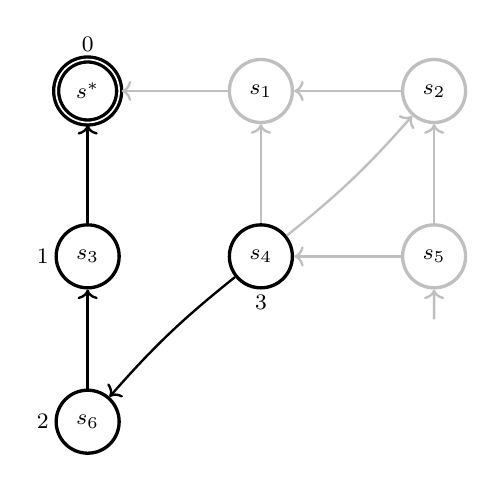
\begin{tikzpicture}
    [
        node distance=21mm and 22mm, on grid, auto, label distance=-0.5mm,
        black_node/.style={circle, draw=black!100, fill=black!0, very thick, minimum height=8mm, minimum width=8mm},
        gray_node/.style={circle, draw=lightgray!100, fill=lightgray!0, very thick, minimum height=8mm, minimum width=8mm},
    ]
        \node[black_node, accepting, label=above:{\footnotesize$0$}] (goal) {\footnotesize$s^*$} ;
        \node[gray_node] (s1) [right = of goal] {\footnotesize$s_{1}$} ;
        \node[gray_node] (s2) [right = of s1] {\footnotesize$s_{2}$} ;
        \node[black_node, label=left:{\footnotesize$1$}] (s3) [below = of goal] {\footnotesize$s_{3}$} ;
        \node[black_node, label=below:{\footnotesize$3$}] (s4) [below = of s1] {\footnotesize$s_{4}$} ;
        \node[gray_node] (s5) [below = of s2] {\footnotesize$s_{5}$} ;
        \node[black_node, label=left:{\footnotesize$2$}] (s6) [below = of s3] {\footnotesize$s_{6}$} ;
        \draw[->, line width=0.3mm, color=lightgray] (s1) to (goal) ;
        \draw[->, line width=0.3mm, color=lightgray] (s2) to (s1) ;
        \draw[->, line width=0.3mm, color=black] (s3) to (goal) ;
        \draw[->, line width=0.3mm, color=black] (s6) to (s3) ;
        \draw[->, line width=0.3mm, color=black] (s4) to[bend right=5] (s6) ;
        \draw[->, line width=0.3mm, color=lightgray] (s4) to (s1) ;
        \draw[->, line width=0.3mm, color=lightgray] (s4) to[bend right=5] (s2) ;
        \draw[->, line width=0.3mm, color=lightgray] (s5) to (s2) ;
        \draw[->, line width=0.3mm, color=lightgray] (s5) to (s4) ;
        \draw[->, line width=0.3mm, color=lightgray] (4.4,-2.9) to (s5) ;
    \end{tikzpicture}
}
\only<2> {
    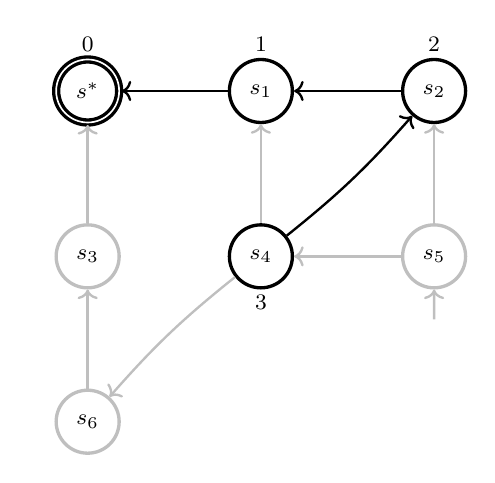
\begin{tikzpicture}
    [
        node distance=21mm and 22mm, on grid, auto, label distance=-0.5mm,
        lightgray_node/.style={circle, draw=lightgray!100, fill=lightgray!0, very thick, minimum height=8mm, minimum width=8mm},
        black_node/.style={circle, draw=black!100, fill=black!0, very thick, minimum height=8mm, minimum width=8mm},
    ]
        \node[black_node, accepting, label=above:{\footnotesize$0$}] (goal) {\footnotesize$s^*$} ;
        \node[black_node, label=above:{\footnotesize$1$}] (s1) [right = of goal] {\footnotesize$s_{1}$} ;
        \node[black_node, label=above:{\footnotesize$2$}] (s2) [right = of s1] {\footnotesize$s_{2}$} ;
        \node[lightgray_node, label=left:{\phantom{\footnotesize$1$}}] (s3) [below = of goal] {\footnotesize$s_{3}$} ;
        \node[black_node, label=below:{\footnotesize$3$}] (s4) [below = of s1] {\footnotesize$s_{4}$} ;
        \node[lightgray_node] (s5) [below = of s2] {\footnotesize$s_{5}$} ;
        \node[lightgray_node] (s6) [below = of s3] {\footnotesize$s_{6}$} ;
        \draw[->, line width=0.3mm, color=black] (s1) to (goal) ;
        \draw[->, line width=0.3mm, color=black] (s2) to (s1) ;
        \draw[->, line width=0.3mm, color=lightgray] (s3) to (goal) ;
        \draw[->, line width=0.3mm, color=lightgray] (s6) to (s3) ;
        \draw[->, line width=0.3mm, color=lightgray] (s4) to[bend right=5] (s6) ;
        \draw[->, line width=0.3mm, color=lightgray] (s4) to (s1) ;
        \draw[->, line width=0.3mm, color=black] (s4) to[bend right=5] (s2) ;
        \draw[->, line width=0.3mm, color=lightgray] (s5) to (s2) ;
        \draw[->, line width=0.3mm, color=lightgray] (s5) to (s4) ;
        \draw[->, line width=0.3mm, color=lightgray] (4.4,-2.9) to (s5) ;
    \end{tikzpicture}
}
\only<3> {
    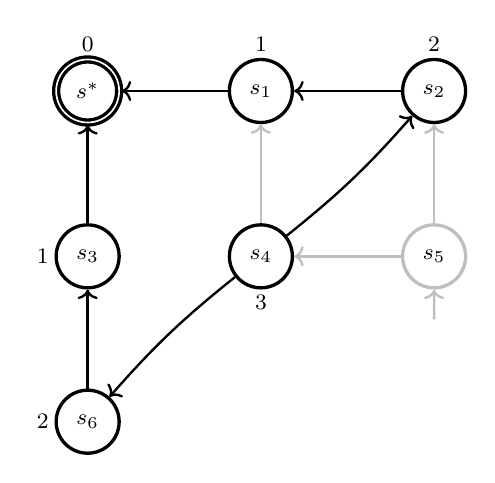
\begin{tikzpicture}
    [
        node distance=21mm and 22mm, on grid, auto, label distance=-0.5mm,
        lightgray_node/.style={circle, draw=lightgray!100, fill=lightgray!0, very thick, minimum height=8mm, minimum width=8mm},
        black_node/.style={circle, draw=black!100, fill=black!0, very thick, minimum height=8mm, minimum width=8mm},
    ]
        \node[black_node, accepting, label=above:{\footnotesize$0$}] (goal) {\footnotesize$s^*$} ;
        \node[black_node, label=above:{\footnotesize$1$}] (s1) [right = of goal] {\footnotesize$s_{1}$} ;
        \node[black_node, label=above:{\footnotesize$2$}] (s2) [right = of s1] {\footnotesize$s_{2}$} ;
        \node[black_node, label=left:{\footnotesize$1$}] (s3) [below = of goal] {\footnotesize$s_{3}$} ;
        \node[black_node, label=below:{\footnotesize$3$}] (s4) [below = of s1] {\footnotesize$s_{4}$} ;
        \node[lightgray_node] (s5) [below = of s2] {\footnotesize$s_{5}$} ;
        \node[black_node, label=left:{\footnotesize$2$}] (s6) [below = of s3] {\footnotesize$s_{6}$} ;
        \draw[->, line width=0.3mm, color=black] (s1) to (goal) ;
        \draw[->, line width=0.3mm, color=black] (s2) to (s1) ;
        \draw[->, line width=0.3mm, color=black] (s3) to (goal) ;
        \draw[->, line width=0.3mm, color=black] (s6) to (s3) ;
        \draw[->, line width=0.3mm, color=black] (s4) to[bend right=5] (s6) ;
        \draw[->, line width=0.3mm, color=lightgray] (s4) to (s1) ;
        \draw[->, line width=0.3mm, color=black] (s4) to[bend right=5] (s2) ;
        \draw[->, line width=0.3mm, color=lightgray] (s5) to (s2) ;
        \draw[->, line width=0.3mm, color=lightgray] (s5) to (s4) ;
        \draw[->, line width=0.3mm, color=lightgray] (4.4,-2.9) to (s5) ;
    \end{tikzpicture}
}
\only<4> {
    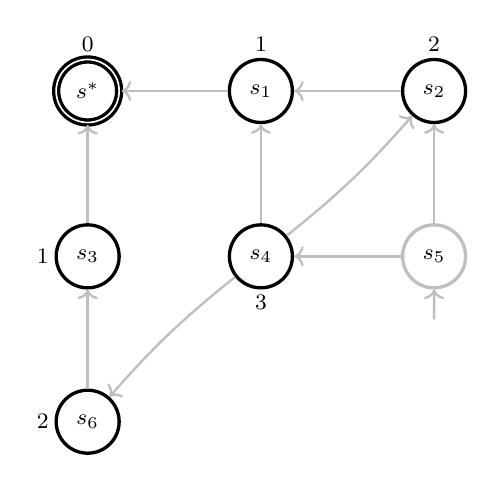
\begin{tikzpicture}
    [
        node distance=21mm and 22mm, on grid, auto, label distance=-0.5mm,
        black_node/.style={circle, draw=black!100, fill=black!0, very thick, minimum height=8mm, minimum width=8mm},
        grey_node/.style={circle, draw=lightgray, fill=black!0, very thick, minimum height=8mm, minimum width=8mm},
    ]
        \node[black_node, accepting, label=above:{\footnotesize$0$}] (goal) {\footnotesize$s^*$} ;
        \node[black_node, label=above:{\footnotesize$1$}] (s1) [right = of goal] {\footnotesize$s_{1}$} ;
        \node[black_node, label=above:{\footnotesize$2$}] (s2) [right = of s1] {\footnotesize$s_{2}$} ;
        \node[black_node, label=left:{\footnotesize$1$}] (s3) [below = of goal] {\footnotesize$s_{3}$} ;
        \node[black_node, label=below:{\footnotesize$3$}] (s4) [below = of s1] {\footnotesize$s_{4}$} ;
        \node[grey_node] (s5) [below = of s2] {\footnotesize$s_{5}$} ;
        \node[black_node, label=left:{\footnotesize$2$}] (s6) [below = of s3] {\footnotesize$s_{6}$} ;
        \draw[->, line width=0.3mm, color=lightgray] (s1) to (goal) ;
        \draw[->, line width=0.3mm, color=lightgray] (s2) to (s1) ;
        \draw[->, line width=0.3mm, color=lightgray] (s3) to (goal) ;
        \draw[->, line width=0.3mm, color=lightgray] (s6) to (s3) ;
        \draw[->, line width=0.3mm, color=lightgray] (s4) to[bend right=5] (s6) ;
        \draw[->, line width=0.3mm, color=lightgray] (s4) to (s1) ;
        \draw[->, line width=0.3mm, color=lightgray] (s4) to[bend right=5] (s2) ;
        \draw[->, line width=0.3mm, color=lightgray] (s5) to (s2) ;
        \draw[->, line width=0.3mm, color=lightgray] (s5) to (s4) ;
        \draw[->, line width=0.3mm, color=lightgray] (4.4,-2.9) to (s5) ;
    \end{tikzpicture}
}
\only<5> {
    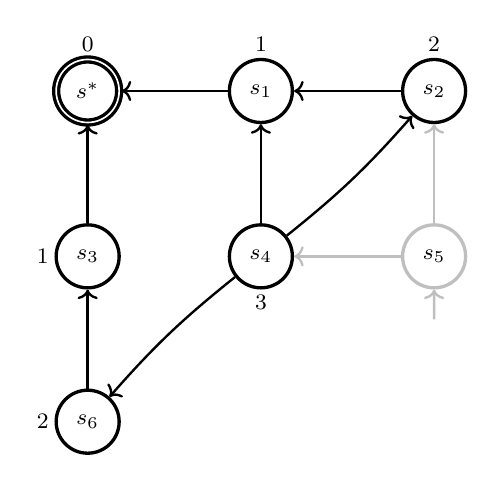
\begin{tikzpicture}
    [
        node distance=21mm and 22mm, on grid, auto, label distance=-0.5mm,
        black_node/.style={circle, draw=black!100, fill=black!0, very thick, minimum height=8mm, minimum width=8mm},
        grey_node/.style={circle, draw=lightgray, fill=black!0, very thick, minimum height=8mm, minimum width=8mm},
    ]
        \node[black_node, accepting, label=above:{\footnotesize$0$}] (goal) {\footnotesize$s^*$} ;
        \node[black_node, label=above:{\footnotesize$1$}] (s1) [right = of goal] {\footnotesize$s_{1}$} ;
        \node[black_node, label=above:{\footnotesize$2$}] (s2) [right = of s1] {\footnotesize$s_{2}$} ;
        \node[black_node, label=left:{\footnotesize$1$}] (s3) [below = of goal] {\footnotesize$s_{3}$} ;
        \node[black_node, label=below:{\footnotesize$3$}] (s4) [below = of s1] {\footnotesize$s_{4}$} ;
        \node[grey_node] (s5) [below = of s2] {\footnotesize$s_{5}$} ;
        \node[black_node, label=left:{\footnotesize$2$}] (s6) [below = of s3] {\footnotesize$s_{6}$} ;
        \draw[->, line width=0.3mm, color=black] (s1) to (goal) ;
        \draw[->, line width=0.3mm, color=black] (s2) to (s1) ;
        \draw[->, line width=0.3mm, color=black] (s3) to (goal) ;
        \draw[->, line width=0.3mm, color=black] (s6) to (s3) ;
        \draw[->, line width=0.3mm, color=black] (s4) to[bend right=5] (s6) ;
        \draw[->, line width=0.3mm, color=black] (s4) to (s1) ;
        \draw[->, line width=0.3mm, color=black] (s4) to[bend right=5] (s2) ;
        \draw[->, line width=0.3mm, color=lightgray] (s5) to (s2) ;
        \draw[->, line width=0.3mm, color=lightgray] (s5) to (s4) ;
        \draw[->, line width=0.3mm, color=lightgray] (4.4,-2.9) to (s5) ;
    \end{tikzpicture}
}
\only<6> {
    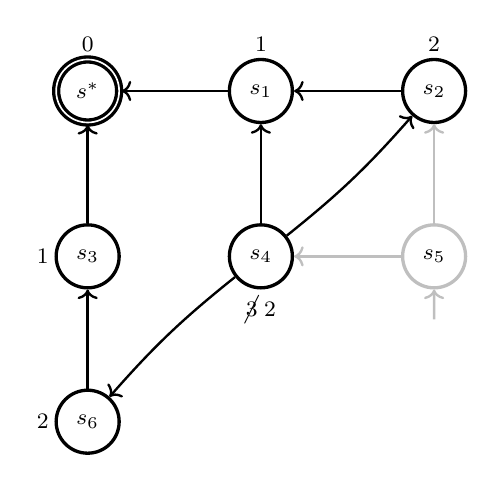
\begin{tikzpicture}
    [
        node distance=21mm and 22mm, on grid, auto, label distance=-0.5mm,
        black_node/.style={circle, draw=black!100, fill=black!0, very thick, minimum height=8mm, minimum width=8mm},
        grey_node/.style={circle, draw=lightgray, fill=black!0, very thick, minimum height=8mm, minimum width=8mm},
    ]
        \node[black_node, accepting, label=above:{\footnotesize$0$}] (goal) {\footnotesize$s^*$} ;
        \node[black_node, label=above:{\footnotesize$1$}] (s1) [right = of goal] {\footnotesize$s_{1}$} ;
        \node[black_node, label=above:{\footnotesize$2$}] (s2) [right = of s1] {\footnotesize$s_{2}$} ;
        \node[black_node, label=left:{\footnotesize$1$}] (s3) [below = of goal] {\footnotesize$s_{3}$} ;
        \node[black_node, label=below:{\footnotesize$\text{\cancel{3}}\;\alert{2}$}] (s4) [below = of s1] {\footnotesize$s_{4}$} ;
        \node[grey_node] (s5) [below = of s2] {\footnotesize$s_{5}$} ;
        \node[black_node, label=left:{\footnotesize$2$}] (s6) [below = of s3] {\footnotesize$s_{6}$} ;
        \draw[->, line width=0.3mm, color=black] (s1) to (goal) ;
        \draw[->, line width=0.3mm, color=black] (s2) to (s1) ;
        \draw[->, line width=0.3mm, color=black] (s3) to (goal) ;
        \draw[->, line width=0.3mm, color=black] (s6) to (s3) ;
        \draw[->, line width=0.3mm, color=black] (s4) to[bend right=5] (s6) ;
        \draw[->, line width=0.3mm, color=black] (s4) to (s1) ;
        \draw[->, line width=0.3mm, color=black] (s4) to[bend right=5] (s2) ;
        \draw[->, line width=0.3mm, color=lightgray] (s5) to (s2) ;
        \draw[->, line width=0.3mm, color=lightgray] (s5) to (s4) ;
        \draw[->, line width=0.3mm, color=lightgray] (4.4,-2.9) to (s5) ;
    \end{tikzpicture}
}
\end{column}
\end{columns}
\end{frame}

\section{Experiments}

\begin{frame}{Experiments}

Systematic analysis of the influence of each feature.
\begin{itemize}
    \item What is the contribution of the sampling algorithm?
    \item What is the impact of the regression limit?
    \item How much do random samples improve the sample set?
    \item How much do our \h-value improvement techniques refine the estimators?
    \item What is the quality of the \h-values produced by the learned heuristics?
    \item Does the quality of the \h-values reflect in the search?
\end{itemize}

\bigskip The experiments were divided into two parts: small state spaces and large state spaces.

\end{frame}

\begin{frame}{Common Settings}
\begin{figure}
    \centering
    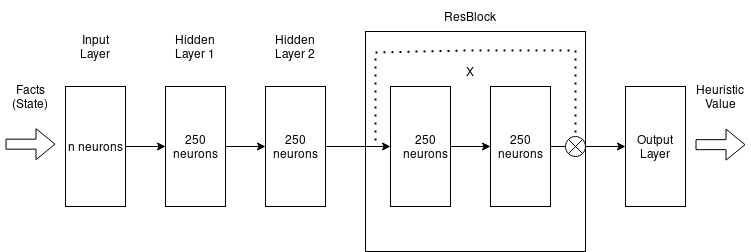
\includegraphics[width=7cm]{figures/resnet.png}
    \caption{Residual network.}
\end{figure}
\begin{itemize}
    \item Same neural network architecture as \citet{ferber2022neural} and \citet{otoole2022sampling}.
    \item Baseline \hnnbase: Random walk sampling, regression limit $L = 200$, and without h-value improvement techniques.
    \item FSM samples $10\,\%$ of the samples with BFS and the rest with RW.
    \item Dataset from \citet{ferber2022neural} moderate tasks.
    \item Each domain: $N$ tasks $\times$ $25$ models $\times$ $50$ initial states.
\end{itemize}
\end{frame}

\subsection{Small State Spaces}

\begin{frame}{Small State Spaces}
\begin{itemize}
    \item Tasks where the forward state space can be enumerated.
    \begin{itemize}
        \item Allows the generation of all states in the state space and their perfect cost-to-goal estimates (\hstar).
        \item Better control and understanding of the behavior of each technique.
    \end{itemize}
    \bigskip
    \item All tasks are solved, so the number of expansions is used as the metric for the quality of the learned heuristic.
    \begin{itemize}
        \item \alert{Fewer expansions} means better heuristics!
    \end{itemize}
\end{itemize}
\end{frame}

\begin{frame}{\small What is the contribution of the sampling algorithm?} % Table 3
\begin{table}[]
\only<1> {
\begin{tabular}{l|rrrr}
    Sampling method & BFS\textsubscript{200} & DFS\textsubscript{200} & RW\textsubscript{200} & FSM\textsubscript{200} \\
    \hline
    Expanded states & 446.72 & 326.66 & 79.78 & 73.12 \\
\end{tabular}
}
\only<2> {
\begin{tabular}{l|rrr}
    Sampling method & & & FSM\textsubscript{200} \\
    \hline
    Expanded states & & \hspace{3.4cm} & 73.12 \\
\end{tabular}
}
\only<3> {
\begin{tabular}{l|rrr}
    Sampling method & & FSM\textsubscript{200} & \\
    \hline
    Expanded states & \hspace{2cm} & 73.12 & \hspace{1cm} \\
\end{tabular}
}
\only<4> {
\begin{tabular}{l|rrr}
    Sampling method & & FSM\textsubscript{200} & \\
    \hline
    Expanded states & \hspace{0.5cm} & 73.12 & \hspace{2cm} \\
\end{tabular}
}
\only<5> {
\begin{tabular}{l|rrr}
    Sampling method & FSM\textsubscript{200} & & \\
    \hline
    Expanded states & 73.12 & & \hspace{2cm} \\
\end{tabular}
}
\end{table}

\only<1> {
\begin{itemize}
    \item BFS and DFS have extreme sample distributions. RW and our approach (FSM) have a balanced sample distribution over the state space.
    \item Blocks expands $5047$ states with BFS and Grid $4102$ with DFS, more than $25$ and $10$ times (resp.) than with the other techniques.
\end{itemize}
}
\only<2-> {
\vspace{3.3cm}
}
\end{frame}

\begin{frame}{\small What is the impact of the regression limit?} % Table 4
\begin{table}[]
\begin{tabular}{l|rrr}
    Sampling method & FSM\textsubscript{\default} & FSM\textsubscript{\facts} & FSM\textsubscript{\meanfx} \\
    \hline
    Expanded states & 73.12 & 63.36 & 69.48 \\
\end{tabular}
\end{table}
\only<1> {
\vspace{3.3cm}
}
\only<2-> {
\begin{itemize}
    \item Our approaches outperform the baseline. \facts has the best performance, but...
    \item \meanfx outperforms the other techniques in 4 of the 7 domains.
    \begin{itemize}
        \item Blocks expands $185$ states, more than twice as many as the other regression limits.
    \end{itemize}
\end{itemize}
\vspace{0.55cm}
}
\end{frame}

\begin{frame}{\small How much do random samples improve the sample set?} % Table 5
\begin{columns}
\begin{column}{0.5\textwidth}
    \begin{table}[]
    \begin{tabular}{l|rr}
        & \multicolumn{2}{c}{Expanded states} \\
        Domain & $0$\% & $20$\% \\
        \hline
        Blocks & 177.88 & \textbf{57.00} \\
        Grid & 124.89 & \textbf{66.52} \\
        N-Puzzle & 89.47 & \textbf{80.93} \\
        Rovers & 17.03 & \textbf{13.45} \\
        Scanalyzer & 55.29 & \textbf{28.34} \\
        Transport & \textbf{22.90} & 25.95 \\
        VisitAll & 30.90 & \textbf{21.78} \\
        \hline
        Geo. mean & 53.91 & 35.13 \\
    \end{tabular}
    \end{table}
\end{column}
\begin{column}{0.5\textwidth}
    \begin{itemize}
        \item Improves performance up to $20$\% of random samples, then degrades.
        \item Up to $50$\% of random samples the expanded states holds close ($35.13$~vs~$38.76$).
    \end{itemize}
\end{column}
\end{columns}
\end{frame}

\begin{frame}{\small How much do our \h-value improvement techniques refine the estimators?} % Table 7
\begin{columns}
\begin{column}{0.5\textwidth}  
    \begin{table}[]
    \begin{tabular}{l|rr}
        & \multicolumn{2}{c}{Mean difference \hstar-\hvalue} \\
        Domain & Baseline & Our approach \\
        \hline
        Blocks & 24.01 & 0.18 \\
        Grid & 13.60 & 0.61 \\
        N-Puzzle & 70.87 & 5.11 \\
        Rovers & 19.92 & 4.88 \\
        Scanalyzer & 81.35 & 1.89 \\
        Transport & 79.06 & 2.44 \\
        VisitAll & 15.80 & 2.15 \\
        \hline
        Geo. mean & 33.45 & 1.60 \\
    \end{tabular}
    \end{table}
\end{column}
\begin{column}{0.4\textwidth}
    \begin{itemize}
        \item All our techniques (FSM, \meanfx, SAI and SUI) improves by $20$~times the approximation of the sample set estimates to \hstar.
        \item Only \meanfx improves the mean difference to $5.56$. Only SAI and SUI improves to $10.95$.
    \end{itemize}
\end{column}
\end{columns}
\end{frame}

\begin{frame}{\small What is the quality of the \h-values produced by the learned heuristics?} % Table 8
\begin{columns}
\begin{column}{0.5\textwidth}
    \begin{table}[]
    \resizebox{\linewidth}{!}{
    \begin{tabular}{l|rr>{\onslide<2->}r<{\onslide}>{\onslide<3->}r<{\onslide}}
         & \multicolumn{4}{>{\onslide<1->}c<{\onslide}}{Mean difference \hstar-\hvalue} \\
        Domain & \hff & \hnnbase & \hnnl{\meanfx} & \hnnrs \\
        \hline
        Blocks & 6.76 & 26.46 & 2.91 & 2.42 \\
        Grid & 3.72 & 26.85 & 2.73 & 9.78 \\
        N-Puzzle & 4.19 & 79.84 & 6.75 & 12.73 \\
        Rovers & 0.17 & 11.08 & 2.98 & 6.35 \\
        Scanalyzer & 2.78 & 106.37 & 2.99 & 9.01 \\
        Transport & 1.13 & 109.77 & 7.05 & 14.89 \\
        VisitAll & 1.31 & 21.55 & 2.21 & 4.74 \\
        \hline
        Geo. mean & 1.84 & 39.80 & 3.57 & 7.40 \\
    \end{tabular}}
    \end{table}
\end{column}
\begin{column}{0.5\textwidth}
    \begin{itemize}
        \item The mean difference \hstar-$h$ over the forward state space of baseline \hnnbase is more than $20$ times greater than \hff.
        \pause
        \item Our approach \hnnl{\meanfx} improves considerably: close to \hff.
        \pause
        \item Adding random samples worsens the mean difference \hstar-$h$.
    \end{itemize}
\end{column}
\end{columns}
\end{frame}

\begin{frame}{\small Does the quality of the \h-values reflect in the search?} % Table 9
\begin{table}[]
\begin{tabular}{l|r>{\onslide<2->}r<{\onslide}>{\onslide<3->}r<{\onslide}>{\onslide<4->}r<{\onslide}>{\onslide<5->}r<{\onslide}}
    Heuristic & \hstar & \hff & \hnnbase & \hnnl{\meanfx} & \hnnrs \\
    \hline
    Expanded states & 14.53 & 38.98 & 81.86 & 53.91 & 35.13 \\
\end{tabular}
\end{table}
\pause \pause \pause
\begin{itemize}
    \item Remains the relative order of quality of estimates over the forward state space.
    \pause
    \item But not. Random samples worsen the quality of estimates but reduce the expanded states.
    \item Our approach with random samples (\hnnrs) outperforms \hff.
\end{itemize}
\end{frame}

\subsection{Large State Spaces}

\begin{frame}{Large State Spaces}
\begin{itemize}
    \item Validate our findings from experiments in small state spaces...
    \begin{itemize}
        \item ...and how does our approach compare with logic-based heuristics and other learned heuristics in the literature?
    \end{itemize}
    \bigskip
    \item Coverage (percentage of solved tasks) is used as the metric for the quality of the learned heuristic.
    \begin{itemize}
        \item \alert{Greater coverage} means better heuristics!
    \end{itemize}
\end{itemize}
\end{frame}

\begin{frame}{Comparison of Heuristic Functions} % Table 12
\begin{columns}
\begin{column}{0.5\textwidth}  
    \begin{table}[]
    \resizebox{\linewidth}{!}{
    \begin{tabular}{l|rrrr}
         & \multicolumn{4}{c}{Coverage (\%)} \\
        Domain & \hff & \hgc & \hnnbase & \hnnrs \\
        \hline
        Blocks & 100.00 & 100.00 & 100.00 & 100.00 \\
        Depot & 94.33 & 80.00 & 57.19 & 89.26 \\
        Grid & 94.00 & 51.00 & 38.11 & 60.33 \\
        N-Puzzle & 92.50 & 4.00 & 13.75 & 86.81 \\
        Pipes-NT & 63.40 & 89.40 & 13.51 & 79.84 \\
        Rovers & 85.50 & 66.00 & 13.53 & 15.39 \\
        Scanalyzer & 100.00 & 100.00 & 59.70 & 73.67 \\
        Storage & 33.00 & 13.50 & 1.94 & 27.67 \\
        Transport & 100.00 & 100.00 & 48.89 & 100.00 \\
        VisitAll & 92.00 & 100.00 & 74.19 & 98.85 \\
        \hline
        Mean & 85.47 & 70.39 & 42.08 & 73.18 \\
    \end{tabular}}
    \end{table}
\end{column}
\begin{column}{0.5\textwidth}
    \begin{itemize}
        \item \hff dominates in most domains.
        \item Our approach \hnnrs improves the baseline \hnnbase by about $31$\%, with competitive coverage in most domains.
        \item Also, outperforms \hgc ($73.18$ vs $70.39$) with higher or equal coverage in $6$ out of $10$ domains.
    \end{itemize}
\end{column}
\end{columns}
\end{frame}

\begin{frame}{Comparison to Other Methods} % Table 13
\begin{table}[]
\begin{tabular}{l|r}
    Technique & Avg. coverage \\
    \hline
    \hboot~\citep{ferber2022neural} & 45.40 \\
    \hnrsl~\citep{otoole2022sampling} & 58.80 \\
    \hnnrs~(Our approach) & 72.82 \\
\end{tabular}
\end{table}
\bigskip
\begin{itemize}
    \item All techniques use the same test dataset and NN architecture.
    \item \hboot uses considerably more computational resources than the other techniques.
    \item Our approach outperforms other techniques.
\end{itemize}
\end{frame}

\section{Conclusion}

\begin{frame}{Conclusion}
\begin{itemize}
    \item A distribution covering various portions of the state space without repeated samples close to the goal works best.
    \item Both the sample distribution and reasonable cost-to-goal estimates contribute to search performance.
    \item The \h-value improvement technique SUI and adaptative rollout limit \meanfx have the most positive impact on sampling quality.
    \item Our approach outperforms \hgc but not \hff.
    \begin{itemize}
        \item \hff has access to the entire model, whereas our approach only uses a minimal part of it.
    \end{itemize}
    \item Approaches with few samples and computational resources can also be efficient.
\end{itemize}
\end{frame}

{\setbeamercolor{palette primary}{fg=white, bg=inf_tertiary}
\begin{frame}[standout]
  Questions?

  \small \email{rvbettker@inf.ufrgs.br}
\end{frame}
}

\begin{frame}[allowframebreaks]{References}
  \bibliography{../references}
  \bibliographystyle{authordate1}
\end{frame}

\end{document}
